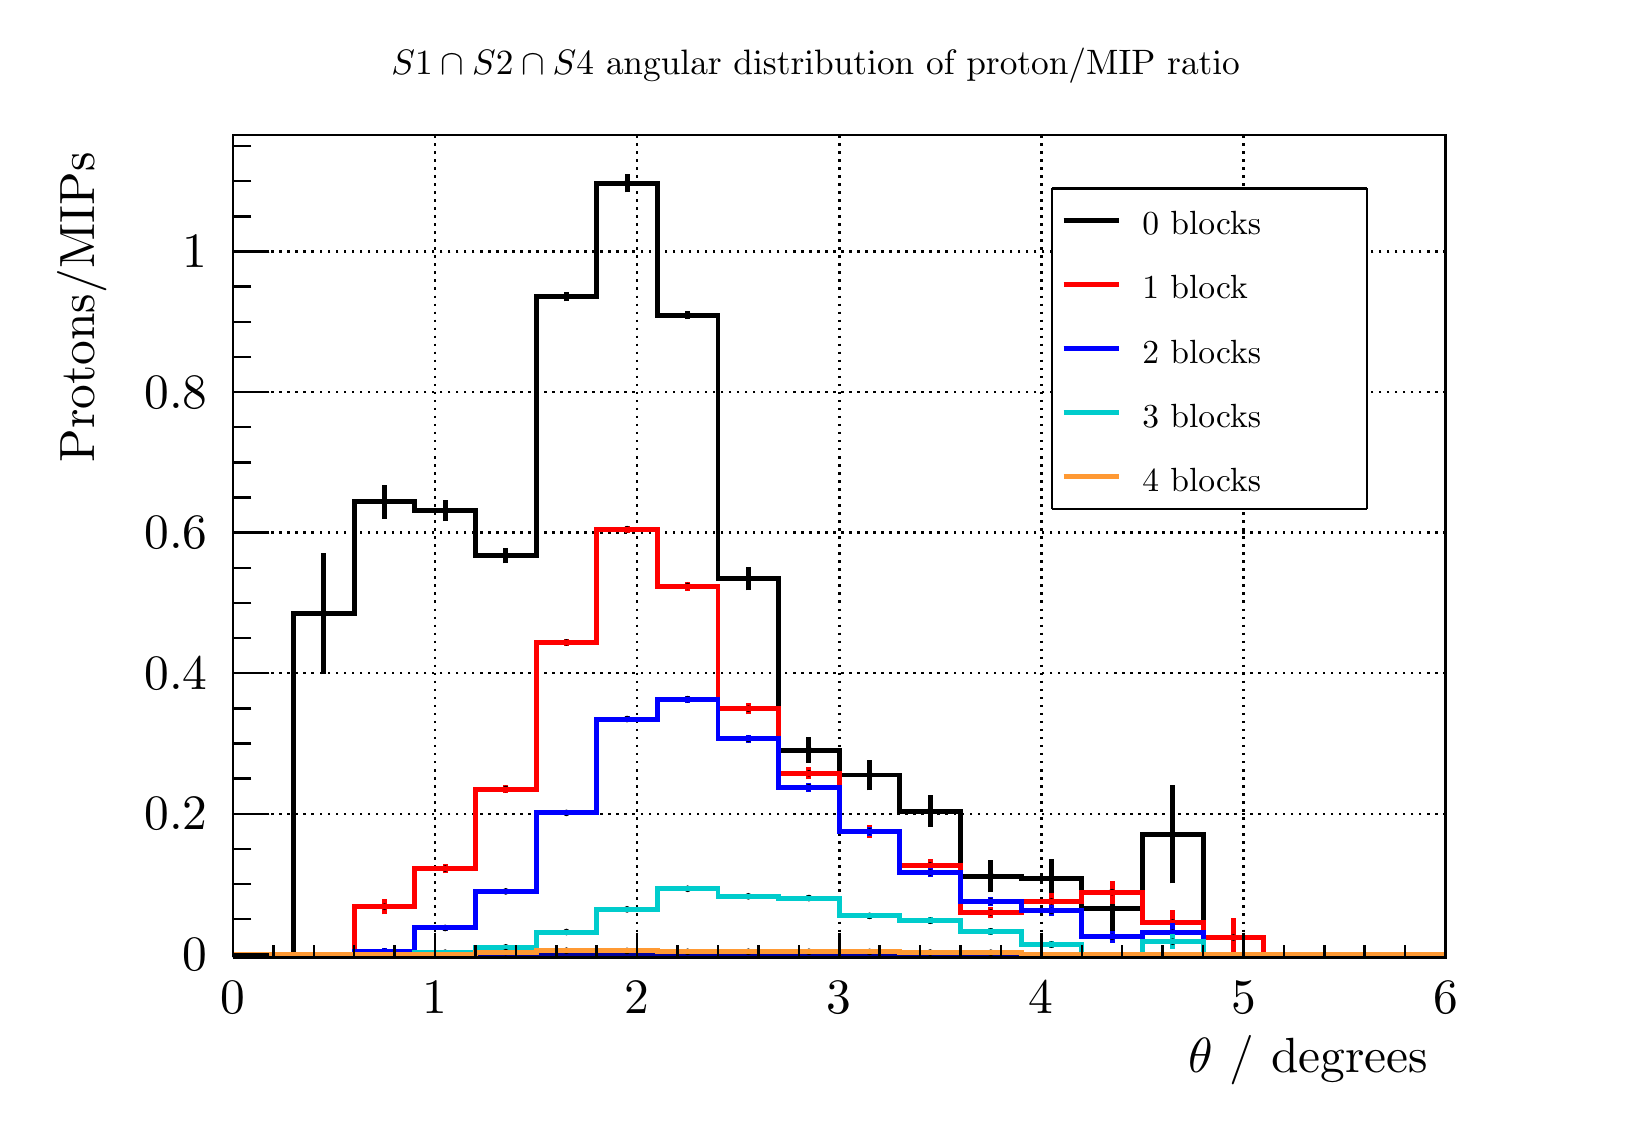
\begin{tikzpicture}
\pgfdeclareplotmark{cross} {
\pgfpathmoveto{\pgfpoint{-0.3\pgfplotmarksize}{\pgfplotmarksize}}
\pgfpathlineto{\pgfpoint{+0.3\pgfplotmarksize}{\pgfplotmarksize}}
\pgfpathlineto{\pgfpoint{+0.3\pgfplotmarksize}{0.3\pgfplotmarksize}}
\pgfpathlineto{\pgfpoint{+1\pgfplotmarksize}{0.3\pgfplotmarksize}}
\pgfpathlineto{\pgfpoint{+1\pgfplotmarksize}{-0.3\pgfplotmarksize}}
\pgfpathlineto{\pgfpoint{+0.3\pgfplotmarksize}{-0.3\pgfplotmarksize}}
\pgfpathlineto{\pgfpoint{+0.3\pgfplotmarksize}{-1.\pgfplotmarksize}}
\pgfpathlineto{\pgfpoint{-0.3\pgfplotmarksize}{-1.\pgfplotmarksize}}
\pgfpathlineto{\pgfpoint{-0.3\pgfplotmarksize}{-0.3\pgfplotmarksize}}
\pgfpathlineto{\pgfpoint{-1.\pgfplotmarksize}{-0.3\pgfplotmarksize}}
\pgfpathlineto{\pgfpoint{-1.\pgfplotmarksize}{0.3\pgfplotmarksize}}
\pgfpathlineto{\pgfpoint{-0.3\pgfplotmarksize}{0.3\pgfplotmarksize}}
\pgfpathclose
\pgfusepathqstroke
}
\pgfdeclareplotmark{cross*} {
\pgfpathmoveto{\pgfpoint{-0.3\pgfplotmarksize}{\pgfplotmarksize}}
\pgfpathlineto{\pgfpoint{+0.3\pgfplotmarksize}{\pgfplotmarksize}}
\pgfpathlineto{\pgfpoint{+0.3\pgfplotmarksize}{0.3\pgfplotmarksize}}
\pgfpathlineto{\pgfpoint{+1\pgfplotmarksize}{0.3\pgfplotmarksize}}
\pgfpathlineto{\pgfpoint{+1\pgfplotmarksize}{-0.3\pgfplotmarksize}}
\pgfpathlineto{\pgfpoint{+0.3\pgfplotmarksize}{-0.3\pgfplotmarksize}}
\pgfpathlineto{\pgfpoint{+0.3\pgfplotmarksize}{-1.\pgfplotmarksize}}
\pgfpathlineto{\pgfpoint{-0.3\pgfplotmarksize}{-1.\pgfplotmarksize}}
\pgfpathlineto{\pgfpoint{-0.3\pgfplotmarksize}{-0.3\pgfplotmarksize}}
\pgfpathlineto{\pgfpoint{-1.\pgfplotmarksize}{-0.3\pgfplotmarksize}}
\pgfpathlineto{\pgfpoint{-1.\pgfplotmarksize}{0.3\pgfplotmarksize}}
\pgfpathlineto{\pgfpoint{-0.3\pgfplotmarksize}{0.3\pgfplotmarksize}}
\pgfpathclose
\pgfusepathqfillstroke
}
\pgfdeclareplotmark{newstar} {
\pgfpathmoveto{\pgfqpoint{0pt}{\pgfplotmarksize}}
\pgfpathlineto{\pgfqpointpolar{44}{0.5\pgfplotmarksize}}
\pgfpathlineto{\pgfqpointpolar{18}{\pgfplotmarksize}}
\pgfpathlineto{\pgfqpointpolar{-20}{0.5\pgfplotmarksize}}
\pgfpathlineto{\pgfqpointpolar{-54}{\pgfplotmarksize}}
\pgfpathlineto{\pgfqpointpolar{-90}{0.5\pgfplotmarksize}}
\pgfpathlineto{\pgfqpointpolar{234}{\pgfplotmarksize}}
\pgfpathlineto{\pgfqpointpolar{198}{0.5\pgfplotmarksize}}
\pgfpathlineto{\pgfqpointpolar{162}{\pgfplotmarksize}}
\pgfpathlineto{\pgfqpointpolar{134}{0.5\pgfplotmarksize}}
\pgfpathclose
\pgfusepathqstroke
}
\pgfdeclareplotmark{newstar*} {
\pgfpathmoveto{\pgfqpoint{0pt}{\pgfplotmarksize}}
\pgfpathlineto{\pgfqpointpolar{44}{0.5\pgfplotmarksize}}
\pgfpathlineto{\pgfqpointpolar{18}{\pgfplotmarksize}}
\pgfpathlineto{\pgfqpointpolar{-20}{0.5\pgfplotmarksize}}
\pgfpathlineto{\pgfqpointpolar{-54}{\pgfplotmarksize}}
\pgfpathlineto{\pgfqpointpolar{-90}{0.5\pgfplotmarksize}}
\pgfpathlineto{\pgfqpointpolar{234}{\pgfplotmarksize}}
\pgfpathlineto{\pgfqpointpolar{198}{0.5\pgfplotmarksize}}
\pgfpathlineto{\pgfqpointpolar{162}{\pgfplotmarksize}}
\pgfpathlineto{\pgfqpointpolar{134}{0.5\pgfplotmarksize}}
\pgfpathclose
\pgfusepathqfillstroke
}
\definecolor{c}{rgb}{1,1,1};
\draw [color=c, fill=c] (0,0) rectangle (20,13.5632);
\draw [color=c, fill=c] (2.6,1.76322) rectangle (18,12.2069);
\definecolor{c}{rgb}{0,0,0};
\draw [c,line width=0.9] (2.6,1.76322) -- (2.6,12.2069) -- (18,12.2069) -- (18,1.76322) -- (2.6,1.76322);
\definecolor{c}{rgb}{1,1,1};
\draw [color=c, fill=c] (2.6,1.76322) rectangle (18,12.2069);
\definecolor{c}{rgb}{0,0,0};
\draw [c,line width=0.9] (2.6,1.76322) -- (2.6,12.2069) -- (18,12.2069) -- (18,1.76322) -- (2.6,1.76322);
\draw [c,line width=0.9] (2.6,1.76322) -- (18,1.76322);
\draw [c,dotted,line width=0.9] (2.6,12.2069) -- (2.6,1.76322);
\draw [c,dotted,line width=0.9] (5.16667,12.2069) -- (5.16667,1.76322);
\draw [c,dotted,line width=0.9] (7.73333,12.2069) -- (7.73333,1.76322);
\draw [c,dotted,line width=0.9] (10.3,12.2069) -- (10.3,1.76322);
\draw [c,dotted,line width=0.9] (12.8667,12.2069) -- (12.8667,1.76322);
\draw [c,dotted,line width=0.9] (15.4333,12.2069) -- (15.4333,1.76322);
\draw [c,dotted,line width=0.9] (18,12.2069) -- (18,1.76322);
\draw [c,line width=0.9] (2.6,1.76322) -- (2.6,12.2069);
\draw [c,dotted,line width=0.9] (18,1.80099) -- (2.6,1.80099);
\draw [c,dotted,line width=0.9] (18,3.58635) -- (2.6,3.58635);
\draw [c,dotted,line width=0.9] (18,5.37171) -- (2.6,5.37171);
\draw [c,dotted,line width=0.9] (18,7.15707) -- (2.6,7.15707);
\draw [c,dotted,line width=0.9] (18,8.94243) -- (2.6,8.94243);
\draw [c,dotted,line width=0.9] (18,10.7278) -- (2.6,10.7278);
\draw [c,dotted,line width=0.9] (18,1.80099) -- (2.6,1.80099);
\draw [c,dotted,line width=0.9] (18,10.7278) -- (2.6,10.7278);
\definecolor{c}{rgb}{0,0,0.6};
\draw [c,line width=0.9] (2.6,1.80099) -- (3.37,1.80099) -- (3.37,1.80099) -- (4.14,1.80099) -- (4.14,1.80099) -- (4.91,1.80099) -- (4.91,1.80099) -- (5.68,1.80099) -- (5.68,1.80099) -- (6.45,1.80099) -- (6.45,1.80099) -- (7.22,1.80099) --
 (7.22,1.80099) -- (7.99,1.80099) -- (7.99,1.80099) -- (8.76,1.80099) -- (8.76,1.80099) -- (9.53,1.80099) -- (9.53,1.80099) -- (10.3,1.80099) -- (10.3,1.80099) -- (11.07,1.80099) -- (11.07,1.80099) -- (11.84,1.80099) -- (11.84,1.80099) --
 (12.61,1.80099) -- (12.61,1.80099) -- (13.38,1.80099) -- (13.38,1.80099) -- (14.15,1.80099) -- (14.15,1.80099) -- (14.92,1.80099) -- (14.92,1.80099) -- (15.69,1.80099) -- (15.69,1.80099) -- (16.46,1.80099) -- (16.46,1.80099) -- (17.23,1.80099) --
 (17.23,1.80099) -- (18,1.80099);
\definecolor{c}{rgb}{0,0,0};
\draw [c,line width=0.9] (2.6,1.76322) -- (18,1.76322);
\draw [anchor= east] (18,0.461149) node[scale=1.78699, color=c, rotate=0]{$\theta$ / degrees};
\draw [c,line width=0.9] (2.6,2.07653) -- (2.6,1.76322);
\draw [c,line width=0.9] (3.11333,1.91987) -- (3.11333,1.76322);
\draw [c,line width=0.9] (3.62667,1.91987) -- (3.62667,1.76322);
\draw [c,line width=0.9] (4.14,1.91987) -- (4.14,1.76322);
\draw [c,line width=0.9] (4.65333,1.91987) -- (4.65333,1.76322);
\draw [c,line width=0.9] (5.16667,2.07653) -- (5.16667,1.76322);
\draw [c,line width=0.9] (5.68,1.91987) -- (5.68,1.76322);
\draw [c,line width=0.9] (6.19333,1.91987) -- (6.19333,1.76322);
\draw [c,line width=0.9] (6.70667,1.91987) -- (6.70667,1.76322);
\draw [c,line width=0.9] (7.22,1.91987) -- (7.22,1.76322);
\draw [c,line width=0.9] (7.73333,2.07653) -- (7.73333,1.76322);
\draw [c,line width=0.9] (8.24667,1.91987) -- (8.24667,1.76322);
\draw [c,line width=0.9] (8.76,1.91987) -- (8.76,1.76322);
\draw [c,line width=0.9] (9.27333,1.91987) -- (9.27333,1.76322);
\draw [c,line width=0.9] (9.78667,1.91987) -- (9.78667,1.76322);
\draw [c,line width=0.9] (10.3,2.07653) -- (10.3,1.76322);
\draw [c,line width=0.9] (10.8133,1.91987) -- (10.8133,1.76322);
\draw [c,line width=0.9] (11.3267,1.91987) -- (11.3267,1.76322);
\draw [c,line width=0.9] (11.84,1.91987) -- (11.84,1.76322);
\draw [c,line width=0.9] (12.3533,1.91987) -- (12.3533,1.76322);
\draw [c,line width=0.9] (12.8667,2.07653) -- (12.8667,1.76322);
\draw [c,line width=0.9] (13.38,1.91987) -- (13.38,1.76322);
\draw [c,line width=0.9] (13.8933,1.91987) -- (13.8933,1.76322);
\draw [c,line width=0.9] (14.4067,1.91987) -- (14.4067,1.76322);
\draw [c,line width=0.9] (14.92,1.91987) -- (14.92,1.76322);
\draw [c,line width=0.9] (15.4333,2.07653) -- (15.4333,1.76322);
\draw [c,line width=0.9] (15.9467,1.91987) -- (15.9467,1.76322);
\draw [c,line width=0.9] (16.46,1.91987) -- (16.46,1.76322);
\draw [c,line width=0.9] (16.9733,1.91987) -- (16.9733,1.76322);
\draw [c,line width=0.9] (17.4867,1.91987) -- (17.4867,1.76322);
\draw [c,line width=0.9] (18,2.07653) -- (18,1.76322);
\draw [anchor=base] (2.6,1.04437) node[scale=1.78699, color=c, rotate=0]{0};
\draw [anchor=base] (5.16667,1.04437) node[scale=1.78699, color=c, rotate=0]{1};
\draw [anchor=base] (7.73333,1.04437) node[scale=1.78699, color=c, rotate=0]{2};
\draw [anchor=base] (10.3,1.04437) node[scale=1.78699, color=c, rotate=0]{3};
\draw [anchor=base] (12.8667,1.04437) node[scale=1.78699, color=c, rotate=0]{4};
\draw [anchor=base] (15.4333,1.04437) node[scale=1.78699, color=c, rotate=0]{5};
\draw [anchor=base] (18,1.04437) node[scale=1.78699, color=c, rotate=0]{6};
\draw [c,line width=0.9] (2.6,1.76322) -- (2.6,12.2069);
\draw [anchor= east] (0.68,12.2069) node[scale=1.78699, color=c, rotate=90]{ Protons/MIPs};
\draw [c,line width=0.9] (3.062,1.80099) -- (2.6,1.80099);
\draw [c,line width=0.9] (2.831,2.24733) -- (2.6,2.24733);
\draw [c,line width=0.9] (2.831,2.69367) -- (2.6,2.69367);
\draw [c,line width=0.9] (2.831,3.14001) -- (2.6,3.14001);
\draw [c,line width=0.9] (3.062,3.58635) -- (2.6,3.58635);
\draw [c,line width=0.9] (2.831,4.03269) -- (2.6,4.03269);
\draw [c,line width=0.9] (2.831,4.47903) -- (2.6,4.47903);
\draw [c,line width=0.9] (2.831,4.92537) -- (2.6,4.92537);
\draw [c,line width=0.9] (3.062,5.37171) -- (2.6,5.37171);
\draw [c,line width=0.9] (2.831,5.81805) -- (2.6,5.81805);
\draw [c,line width=0.9] (2.831,6.26439) -- (2.6,6.26439);
\draw [c,line width=0.9] (2.831,6.71073) -- (2.6,6.71073);
\draw [c,line width=0.9] (3.062,7.15707) -- (2.6,7.15707);
\draw [c,line width=0.9] (2.831,7.60341) -- (2.6,7.60341);
\draw [c,line width=0.9] (2.831,8.04975) -- (2.6,8.04975);
\draw [c,line width=0.9] (2.831,8.49609) -- (2.6,8.49609);
\draw [c,line width=0.9] (3.062,8.94243) -- (2.6,8.94243);
\draw [c,line width=0.9] (2.831,9.38877) -- (2.6,9.38877);
\draw [c,line width=0.9] (2.831,9.83511) -- (2.6,9.83511);
\draw [c,line width=0.9] (2.831,10.2815) -- (2.6,10.2815);
\draw [c,line width=0.9] (3.062,10.7278) -- (2.6,10.7278);
\draw [c,line width=0.9] (3.062,1.80099) -- (2.6,1.80099);
\draw [c,line width=0.9] (3.062,10.7278) -- (2.6,10.7278);
\draw [c,line width=0.9] (2.831,11.1741) -- (2.6,11.1741);
\draw [c,line width=0.9] (2.831,11.6205) -- (2.6,11.6205);
\draw [c,line width=0.9] (2.831,12.0668) -- (2.6,12.0668);
\draw [anchor= east] (2.5,1.80099) node[scale=1.78699, color=c, rotate=0]{0};
\draw [anchor= east] (2.5,3.58635) node[scale=1.78699, color=c, rotate=0]{0.2};
\draw [anchor= east] (2.5,5.37171) node[scale=1.78699, color=c, rotate=0]{0.4};
\draw [anchor= east] (2.5,7.15707) node[scale=1.78699, color=c, rotate=0]{0.6};
\draw [anchor= east] (2.5,8.94243) node[scale=1.78699, color=c, rotate=0]{0.8};
\draw [anchor= east] (2.5,10.7278) node[scale=1.78699, color=c, rotate=0]{1};
\draw [c,line width=1.8] (3.755,5.35705) -- (3.755,6.12779);
\draw [c,line width=1.8] (3.755,6.12779) -- (3.755,6.89852);
\foreach \P in {(3.755,6.12779)}{\draw[mark options={color=c,fill=c},mark size=2.402402pt,mark=*,mark size=1pt] plot coordinates {\P};}
\draw [c,line width=1.8] (4.525,7.33357) -- (4.525,7.55069);
\draw [c,line width=1.8] (4.525,7.55069) -- (4.525,7.76781);
\foreach \P in {(4.525,7.55069)}{\draw[mark options={color=c,fill=c},mark size=2.402402pt,mark=*,mark size=1pt] plot coordinates {\P};}
\draw [c,line width=1.8] (5.295,7.30262) -- (5.295,7.43563);
\draw [c,line width=1.8] (5.295,7.43563) -- (5.295,7.56865);
\foreach \P in {(5.295,7.43563)}{\draw[mark options={color=c,fill=c},mark size=2.402402pt,mark=*,mark size=1pt] plot coordinates {\P};}
\draw [c,line width=1.8] (6.065,6.76821) -- (6.065,6.86574);
\draw [c,line width=1.8] (6.065,6.86574) -- (6.065,6.96326);
\foreach \P in {(6.065,6.86574)}{\draw[mark options={color=c,fill=c},mark size=2.402402pt,mark=*,mark size=1pt] plot coordinates {\P};}
\draw [c,line width=1.8] (6.835,10.0927) -- (6.835,10.1505);
\draw [c,line width=1.8] (6.835,10.1505) -- (6.835,10.2083);
\foreach \P in {(6.835,10.1505)}{\draw[mark options={color=c,fill=c},mark size=2.402402pt,mark=*,mark size=1pt] plot coordinates {\P};}
\draw [c,line width=1.8] (7.605,11.4789) -- (7.605,11.5951);
\draw [c,line width=1.8] (7.605,11.5951) -- (7.605,11.7114);
\foreach \P in {(7.605,11.5951)}{\draw[mark options={color=c,fill=c},mark size=2.402402pt,mark=*,mark size=1pt] plot coordinates {\P};}
\draw [c,line width=1.8] (8.375,9.86813) -- (8.375,9.91934);
\draw [c,line width=1.8] (8.375,9.91934) -- (8.375,9.97055);
\foreach \P in {(8.375,9.91934)}{\draw[mark options={color=c,fill=c},mark size=2.402402pt,mark=*,mark size=1pt] plot coordinates {\P};}
\draw [c,line width=1.8] (9.145,6.42489) -- (9.145,6.57357);
\draw [c,line width=1.8] (9.145,6.57357) -- (9.145,6.72224);
\foreach \P in {(9.145,6.57357)}{\draw[mark options={color=c,fill=c},mark size=2.402402pt,mark=*,mark size=1pt] plot coordinates {\P};}
\draw [c,line width=1.8] (9.915,4.23337) -- (9.915,4.39551);
\draw [c,line width=1.8] (9.915,4.39551) -- (9.915,4.55766);
\foreach \P in {(9.915,4.39551)}{\draw[mark options={color=c,fill=c},mark size=2.402402pt,mark=*,mark size=1pt] plot coordinates {\P};}
\draw [c,line width=1.8] (10.685,3.88461) -- (10.685,4.07908);
\draw [c,line width=1.8] (10.685,4.07908) -- (10.685,4.27354);
\foreach \P in {(10.685,4.07908)}{\draw[mark options={color=c,fill=c},mark size=2.402402pt,mark=*,mark size=1pt] plot coordinates {\P};}
\draw [c,line width=1.8] (11.455,3.42304) -- (11.455,3.62098);
\draw [c,line width=1.8] (11.455,3.62098) -- (11.455,3.81892);
\foreach \P in {(11.455,3.62098)}{\draw[mark options={color=c,fill=c},mark size=2.402402pt,mark=*,mark size=1pt] plot coordinates {\P};}
\draw [c,line width=1.8] (12.225,2.58946) -- (12.225,2.79587);
\draw [c,line width=1.8] (12.225,2.79587) -- (12.225,3.00227);
\foreach \P in {(12.225,2.79587)}{\draw[mark options={color=c,fill=c},mark size=2.402402pt,mark=*,mark size=1pt] plot coordinates {\P};}
\draw [c,line width=1.8] (12.995,2.5248) -- (12.995,2.76957);
\draw [c,line width=1.8] (12.995,2.76957) -- (12.995,3.01435);
\foreach \P in {(12.995,2.76957)}{\draw[mark options={color=c,fill=c},mark size=2.402402pt,mark=*,mark size=1pt] plot coordinates {\P};}
\draw [c,line width=1.8] (13.765,2.06428) -- (13.765,2.38414);
\draw [c,line width=1.8] (13.765,2.38414) -- (13.765,2.704);
\foreach \P in {(13.765,2.38414)}{\draw[mark options={color=c,fill=c},mark size=2.402402pt,mark=*,mark size=1pt] plot coordinates {\P};}
\draw [c,line width=1.8] (14.535,2.70225) -- (14.535,3.32727);
\draw [c,line width=1.8] (14.535,3.32727) -- (14.535,3.95228);
\foreach \P in {(14.535,3.32727)}{\draw[mark options={color=c,fill=c},mark size=2.402402pt,mark=*,mark size=1pt] plot coordinates {\P};}
\draw [c,line width=1.8] (2.6,1.80099) -- (3.37,1.80099) -- (3.37,6.12779) -- (4.14,6.12779) -- (4.14,7.55069) -- (4.91,7.55069) -- (4.91,7.43563) -- (5.68,7.43563) -- (5.68,6.86574) -- (6.45,6.86574) -- (6.45,10.1505) -- (7.22,10.1505) --
 (7.22,11.5951) -- (7.99,11.5951) -- (7.99,9.91934) -- (8.76,9.91934) -- (8.76,6.57357) -- (9.53,6.57357) -- (9.53,4.39551) -- (10.3,4.39551) -- (10.3,4.07908) -- (11.07,4.07908) -- (11.07,3.62098) -- (11.84,3.62098) -- (11.84,2.79587) --
 (12.61,2.79587) -- (12.61,2.76957) -- (13.38,2.76957) -- (13.38,2.38414) -- (14.15,2.38414) -- (14.15,3.32727) -- (14.92,3.32727) -- (14.92,1.80099) -- (15.69,1.80099) -- (15.69,1.80099) -- (16.46,1.80099) -- (16.46,1.80099) -- (17.23,1.80099) --
 (17.23,1.80099) -- (18,1.80099);
\definecolor{c}{rgb}{1,0,0};
\draw [c,line width=1.8] (4.525,2.3103) -- (4.525,2.40691);
\draw [c,line width=1.8] (4.525,2.40691) -- (4.525,2.50352);
\definecolor{c}{rgb}{0,0,0};
\foreach \P in {(4.525,2.40691)}{\draw[mark options={color=c,fill=c},mark size=2.402402pt,mark=*,mark size=1pt] plot coordinates {\P};}
\definecolor{c}{rgb}{1,0,0};
\draw [c,line width=1.8] (5.295,2.83129) -- (5.295,2.89079);
\draw [c,line width=1.8] (5.295,2.89079) -- (5.295,2.95028);
\definecolor{c}{rgb}{0,0,0};
\foreach \P in {(5.295,2.89079)}{\draw[mark options={color=c,fill=c},mark size=2.402402pt,mark=*,mark size=1pt] plot coordinates {\P};}
\definecolor{c}{rgb}{1,0,0};
\draw [c,line width=1.8] (6.065,3.85433) -- (6.065,3.90119);
\draw [c,line width=1.8] (6.065,3.90119) -- (6.065,3.94804);
\definecolor{c}{rgb}{0,0,0};
\foreach \P in {(6.065,3.90119)}{\draw[mark options={color=c,fill=c},mark size=2.402402pt,mark=*,mark size=1pt] plot coordinates {\P};}
\definecolor{c}{rgb}{1,0,0};
\draw [c,line width=1.8] (6.835,5.71812) -- (6.835,5.76308);
\draw [c,line width=1.8] (6.835,5.76308) -- (6.835,5.80805);
\definecolor{c}{rgb}{0,0,0};
\foreach \P in {(6.835,5.76308)}{\draw[mark options={color=c,fill=c},mark size=2.402402pt,mark=*,mark size=1pt] plot coordinates {\P};}
\definecolor{c}{rgb}{1,0,0};
\draw [c,line width=1.8] (7.605,7.15528) -- (7.605,7.20102);
\draw [c,line width=1.8] (7.605,7.20102) -- (7.605,7.24677);
\definecolor{c}{rgb}{0,0,0};
\foreach \P in {(7.605,7.20102)}{\draw[mark options={color=c,fill=c},mark size=2.402402pt,mark=*,mark size=1pt] plot coordinates {\P};}
\definecolor{c}{rgb}{1,0,0};
\draw [c,line width=1.8] (8.375,6.42217) -- (8.375,6.47898);
\draw [c,line width=1.8] (8.375,6.47898) -- (8.375,6.5358);
\definecolor{c}{rgb}{0,0,0};
\foreach \P in {(8.375,6.47898)}{\draw[mark options={color=c,fill=c},mark size=2.402402pt,mark=*,mark size=1pt] plot coordinates {\P};}
\definecolor{c}{rgb}{1,0,0};
\draw [c,line width=1.8] (9.145,4.85006) -- (9.145,4.92074);
\draw [c,line width=1.8] (9.145,4.92074) -- (9.145,4.99142);
\definecolor{c}{rgb}{0,0,0};
\foreach \P in {(9.145,4.92074)}{\draw[mark options={color=c,fill=c},mark size=2.402402pt,mark=*,mark size=1pt] plot coordinates {\P};}
\definecolor{c}{rgb}{1,0,0};
\draw [c,line width=1.8] (9.915,4.0238) -- (9.915,4.10059);
\draw [c,line width=1.8] (9.915,4.10059) -- (9.915,4.17739);
\definecolor{c}{rgb}{0,0,0};
\foreach \P in {(9.915,4.10059)}{\draw[mark options={color=c,fill=c},mark size=2.402402pt,mark=*,mark size=1pt] plot coordinates {\P};}
\definecolor{c}{rgb}{1,0,0};
\draw [c,line width=1.8] (10.685,3.2846) -- (10.685,3.36739);
\draw [c,line width=1.8] (10.685,3.36739) -- (10.685,3.45018);
\definecolor{c}{rgb}{0,0,0};
\foreach \P in {(10.685,3.36739)}{\draw[mark options={color=c,fill=c},mark size=2.402402pt,mark=*,mark size=1pt] plot coordinates {\P};}
\definecolor{c}{rgb}{1,0,0};
\draw [c,line width=1.8] (11.455,2.84657) -- (11.455,2.9316);
\draw [c,line width=1.8] (11.455,2.9316) -- (11.455,3.01663);
\definecolor{c}{rgb}{0,0,0};
\foreach \P in {(11.455,2.9316)}{\draw[mark options={color=c,fill=c},mark size=2.402402pt,mark=*,mark size=1pt] plot coordinates {\P};}
\definecolor{c}{rgb}{1,0,0};
\draw [c,line width=1.8] (12.225,2.26143) -- (12.225,2.33414);
\draw [c,line width=1.8] (12.225,2.33414) -- (12.225,2.40685);
\definecolor{c}{rgb}{0,0,0};
\foreach \P in {(12.225,2.33414)}{\draw[mark options={color=c,fill=c},mark size=2.402402pt,mark=*,mark size=1pt] plot coordinates {\P};}
\definecolor{c}{rgb}{1,0,0};
\draw [c,line width=1.8] (12.995,2.37079) -- (12.995,2.47402);
\draw [c,line width=1.8] (12.995,2.47402) -- (12.995,2.57725);
\definecolor{c}{rgb}{0,0,0};
\foreach \P in {(12.995,2.47402)}{\draw[mark options={color=c,fill=c},mark size=2.402402pt,mark=*,mark size=1pt] plot coordinates {\P};}
\definecolor{c}{rgb}{1,0,0};
\draw [c,line width=1.8] (13.765,2.4461) -- (13.765,2.59144);
\draw [c,line width=1.8] (13.765,2.59144) -- (13.765,2.73678);
\definecolor{c}{rgb}{0,0,0};
\foreach \P in {(13.765,2.59144)}{\draw[mark options={color=c,fill=c},mark size=2.402402pt,mark=*,mark size=1pt] plot coordinates {\P};}
\definecolor{c}{rgb}{1,0,0};
\draw [c,line width=1.8] (14.535,2.04767) -- (14.535,2.20607);
\draw [c,line width=1.8] (14.535,2.20607) -- (14.535,2.36446);
\definecolor{c}{rgb}{0,0,0};
\foreach \P in {(14.535,2.20607)}{\draw[mark options={color=c,fill=c},mark size=2.402402pt,mark=*,mark size=1pt] plot coordinates {\P};}
\definecolor{c}{rgb}{1,0,0};
\draw [c,line width=1.8] (15.305,1.76322) -- (15.305,2.01519);
\draw [c,line width=1.8] (15.305,2.01519) -- (15.305,2.26717);
\definecolor{c}{rgb}{0,0,0};
\foreach \P in {(15.305,2.01519)}{\draw[mark options={color=c,fill=c},mark size=2.402402pt,mark=*,mark size=1pt] plot coordinates {\P};}
\definecolor{c}{rgb}{1,0,0};
\draw [c,line width=1.8] (2.6,1.80099) -- (3.37,1.80099) -- (3.37,1.80099) -- (4.14,1.80099) -- (4.14,2.40691) -- (4.91,2.40691) -- (4.91,2.89079) -- (5.68,2.89079) -- (5.68,3.90119) -- (6.45,3.90119) -- (6.45,5.76308) -- (7.22,5.76308) --
 (7.22,7.20102) -- (7.99,7.20102) -- (7.99,6.47898) -- (8.76,6.47898) -- (8.76,4.92074) -- (9.53,4.92074) -- (9.53,4.10059) -- (10.3,4.10059) -- (10.3,3.36739) -- (11.07,3.36739) -- (11.07,2.9316) -- (11.84,2.9316) -- (11.84,2.33414) --
 (12.61,2.33414) -- (12.61,2.47402) -- (13.38,2.47402) -- (13.38,2.59144) -- (14.15,2.59144) -- (14.15,2.20607) -- (14.92,2.20607) -- (14.92,2.01519) -- (15.69,2.01519) -- (15.69,1.80099) -- (16.46,1.80099) -- (16.46,1.80099) -- (17.23,1.80099) --
 (17.23,1.80099) -- (18,1.80099);
\definecolor{c}{rgb}{0,0,1};
\draw [c,line width=1.8] (4.525,1.77992) -- (4.525,1.83412);
\draw [c,line width=1.8] (4.525,1.83412) -- (4.525,1.88832);
\definecolor{c}{rgb}{0,0,0};
\foreach \P in {(4.525,1.83412)}{\draw[mark options={color=c,fill=c},mark size=2.402402pt,mark=*,mark size=1pt] plot coordinates {\P};}
\definecolor{c}{rgb}{0,0,1};
\draw [c,line width=1.8] (5.295,2.10312) -- (5.295,2.13654);
\draw [c,line width=1.8] (5.295,2.13654) -- (5.295,2.16995);
\definecolor{c}{rgb}{0,0,0};
\foreach \P in {(5.295,2.13654)}{\draw[mark options={color=c,fill=c},mark size=2.402402pt,mark=*,mark size=1pt] plot coordinates {\P};}
\definecolor{c}{rgb}{0,0,1};
\draw [c,line width=1.8] (6.065,2.57279) -- (6.065,2.60114);
\draw [c,line width=1.8] (6.065,2.60114) -- (6.065,2.62949);
\definecolor{c}{rgb}{0,0,0};
\foreach \P in {(6.065,2.60114)}{\draw[mark options={color=c,fill=c},mark size=2.402402pt,mark=*,mark size=1pt] plot coordinates {\P};}
\definecolor{c}{rgb}{0,0,1};
\draw [c,line width=1.8] (6.835,3.56624) -- (6.835,3.59803);
\draw [c,line width=1.8] (6.835,3.59803) -- (6.835,3.62981);
\definecolor{c}{rgb}{0,0,0};
\foreach \P in {(6.835,3.59803)}{\draw[mark options={color=c,fill=c},mark size=2.402402pt,mark=*,mark size=1pt] plot coordinates {\P};}
\definecolor{c}{rgb}{0,0,1};
\draw [c,line width=1.8] (7.605,4.75253) -- (7.605,4.78983);
\draw [c,line width=1.8] (7.605,4.78983) -- (7.605,4.82714);
\definecolor{c}{rgb}{0,0,0};
\foreach \P in {(7.605,4.78983)}{\draw[mark options={color=c,fill=c},mark size=2.402402pt,mark=*,mark size=1pt] plot coordinates {\P};}
\definecolor{c}{rgb}{0,0,1};
\draw [c,line width=1.8] (8.375,4.99759) -- (8.375,5.042);
\draw [c,line width=1.8] (8.375,5.042) -- (8.375,5.08642);
\definecolor{c}{rgb}{0,0,0};
\foreach \P in {(8.375,5.042)}{\draw[mark options={color=c,fill=c},mark size=2.402402pt,mark=*,mark size=1pt] plot coordinates {\P};}
\definecolor{c}{rgb}{0,0,1};
\draw [c,line width=1.8] (9.145,4.48496) -- (9.145,4.53648);
\draw [c,line width=1.8] (9.145,4.53648) -- (9.145,4.588);
\definecolor{c}{rgb}{0,0,0};
\foreach \P in {(9.145,4.53648)}{\draw[mark options={color=c,fill=c},mark size=2.402402pt,mark=*,mark size=1pt] plot coordinates {\P};}
\definecolor{c}{rgb}{0,0,1};
\draw [c,line width=1.8] (9.915,3.86841) -- (9.915,3.92463);
\draw [c,line width=1.8] (9.915,3.92463) -- (9.915,3.98085);
\definecolor{c}{rgb}{0,0,0};
\foreach \P in {(9.915,3.92463)}{\draw[mark options={color=c,fill=c},mark size=2.402402pt,mark=*,mark size=1pt] plot coordinates {\P};}
\definecolor{c}{rgb}{0,0,1};
\draw [c,line width=1.8] (10.685,3.30396) -- (10.685,3.36389);
\draw [c,line width=1.8] (10.685,3.36389) -- (10.685,3.42383);
\definecolor{c}{rgb}{0,0,0};
\foreach \P in {(10.685,3.36389)}{\draw[mark options={color=c,fill=c},mark size=2.402402pt,mark=*,mark size=1pt] plot coordinates {\P};}
\definecolor{c}{rgb}{0,0,1};
\draw [c,line width=1.8] (11.455,2.78176) -- (11.455,2.84168);
\draw [c,line width=1.8] (11.455,2.84168) -- (11.455,2.9016);
\definecolor{c}{rgb}{0,0,0};
\foreach \P in {(11.455,2.84168)}{\draw[mark options={color=c,fill=c},mark size=2.402402pt,mark=*,mark size=1pt] plot coordinates {\P};}
\definecolor{c}{rgb}{0,0,1};
\draw [c,line width=1.8] (12.225,2.41229) -- (12.225,2.47409);
\draw [c,line width=1.8] (12.225,2.47409) -- (12.225,2.5359);
\definecolor{c}{rgb}{0,0,0};
\foreach \P in {(12.225,2.47409)}{\draw[mark options={color=c,fill=c},mark size=2.402402pt,mark=*,mark size=1pt] plot coordinates {\P};}
\definecolor{c}{rgb}{0,0,1};
\draw [c,line width=1.8] (12.995,2.28351) -- (12.995,2.35366);
\draw [c,line width=1.8] (12.995,2.35366) -- (12.995,2.42381);
\definecolor{c}{rgb}{0,0,0};
\foreach \P in {(12.995,2.35366)}{\draw[mark options={color=c,fill=c},mark size=2.402402pt,mark=*,mark size=1pt] plot coordinates {\P};}
\definecolor{c}{rgb}{0,0,1};
\draw [c,line width=1.8] (13.765,1.94671) -- (13.765,2.02366);
\draw [c,line width=1.8] (13.765,2.02366) -- (13.765,2.10061);
\definecolor{c}{rgb}{0,0,0};
\foreach \P in {(13.765,2.02366)}{\draw[mark options={color=c,fill=c},mark size=2.402402pt,mark=*,mark size=1pt] plot coordinates {\P};}
\definecolor{c}{rgb}{0,0,1};
\draw [c,line width=1.8] (14.535,1.96006) -- (14.535,2.07811);
\draw [c,line width=1.8] (14.535,2.07811) -- (14.535,2.19615);
\definecolor{c}{rgb}{0,0,0};
\foreach \P in {(14.535,2.07811)}{\draw[mark options={color=c,fill=c},mark size=2.402402pt,mark=*,mark size=1pt] plot coordinates {\P};}
\definecolor{c}{rgb}{0,0,1};
\draw [c,line width=1.8] (2.6,1.80099) -- (3.37,1.80099) -- (3.37,1.80099) -- (4.14,1.80099) -- (4.14,1.83412) -- (4.91,1.83412) -- (4.91,2.13654) -- (5.68,2.13654) -- (5.68,2.60114) -- (6.45,2.60114) -- (6.45,3.59803) -- (7.22,3.59803) --
 (7.22,4.78983) -- (7.99,4.78983) -- (7.99,5.042) -- (8.76,5.042) -- (8.76,4.53648) -- (9.53,4.53648) -- (9.53,3.92463) -- (10.3,3.92463) -- (10.3,3.36389) -- (11.07,3.36389) -- (11.07,2.84168) -- (11.84,2.84168) -- (11.84,2.47409) -- (12.61,2.47409)
 -- (12.61,2.35366) -- (13.38,2.35366) -- (13.38,2.02366) -- (14.15,2.02366) -- (14.15,2.07811) -- (14.92,2.07811) -- (14.92,1.80099) -- (15.69,1.80099) -- (15.69,1.80099) -- (16.46,1.80099) -- (16.46,1.80099) -- (17.23,1.80099) -- (17.23,1.80099) --
 (18,1.80099);
\definecolor{c}{rgb}{0,0.8,0.8};
\draw [c,line width=1.8] (5.295,1.80369) -- (5.295,1.82223);
\draw [c,line width=1.8] (5.295,1.82223) -- (5.295,1.84077);
\definecolor{c}{rgb}{0,0,0};
\foreach \P in {(5.295,1.82223)}{\draw[mark options={color=c,fill=c},mark size=2.402402pt,mark=*,mark size=1pt] plot coordinates {\P};}
\definecolor{c}{rgb}{0,0.8,0.8};
\draw [c,line width=1.8] (6.065,1.87736) -- (6.065,1.8901);
\draw [c,line width=1.8] (6.065,1.8901) -- (6.065,1.90285);
\definecolor{c}{rgb}{0,0,0};
\foreach \P in {(6.065,1.8901)}{\draw[mark options={color=c,fill=c},mark size=2.402402pt,mark=*,mark size=1pt] plot coordinates {\P};}
\definecolor{c}{rgb}{0,0.8,0.8};
\draw [c,line width=1.8] (6.835,2.06766) -- (6.835,2.08505);
\draw [c,line width=1.8] (6.835,2.08505) -- (6.835,2.10245);
\definecolor{c}{rgb}{0,0,0};
\foreach \P in {(6.835,2.08505)}{\draw[mark options={color=c,fill=c},mark size=2.402402pt,mark=*,mark size=1pt] plot coordinates {\P};}
\definecolor{c}{rgb}{0,0.8,0.8};
\draw [c,line width=1.8] (7.605,2.35106) -- (7.605,2.37308);
\draw [c,line width=1.8] (7.605,2.37308) -- (7.605,2.39511);
\definecolor{c}{rgb}{0,0,0};
\foreach \P in {(7.605,2.37308)}{\draw[mark options={color=c,fill=c},mark size=2.402402pt,mark=*,mark size=1pt] plot coordinates {\P};}
\definecolor{c}{rgb}{0,0.8,0.8};
\draw [c,line width=1.8] (8.375,2.60435) -- (8.375,2.63408);
\draw [c,line width=1.8] (8.375,2.63408) -- (8.375,2.66381);
\definecolor{c}{rgb}{0,0,0};
\foreach \P in {(8.375,2.63408)}{\draw[mark options={color=c,fill=c},mark size=2.402402pt,mark=*,mark size=1pt] plot coordinates {\P};}
\definecolor{c}{rgb}{0,0.8,0.8};
\draw [c,line width=1.8] (9.145,2.50436) -- (9.145,2.53863);
\draw [c,line width=1.8] (9.145,2.53863) -- (9.145,2.57291);
\definecolor{c}{rgb}{0,0,0};
\foreach \P in {(9.145,2.53863)}{\draw[mark options={color=c,fill=c},mark size=2.402402pt,mark=*,mark size=1pt] plot coordinates {\P};}
\definecolor{c}{rgb}{0,0.8,0.8};
\draw [c,line width=1.8] (9.915,2.47528) -- (9.915,2.51596);
\draw [c,line width=1.8] (9.915,2.51596) -- (9.915,2.55663);
\definecolor{c}{rgb}{0,0,0};
\foreach \P in {(9.915,2.51596)}{\draw[mark options={color=c,fill=c},mark size=2.402402pt,mark=*,mark size=1pt] plot coordinates {\P};}
\definecolor{c}{rgb}{0,0.8,0.8};
\draw [c,line width=1.8] (10.685,2.25227) -- (10.685,2.29032);
\draw [c,line width=1.8] (10.685,2.29032) -- (10.685,2.32838);
\definecolor{c}{rgb}{0,0,0};
\foreach \P in {(10.685,2.29032)}{\draw[mark options={color=c,fill=c},mark size=2.402402pt,mark=*,mark size=1pt] plot coordinates {\P};}
\definecolor{c}{rgb}{0,0.8,0.8};
\draw [c,line width=1.8] (11.455,2.18667) -- (11.455,2.22834);
\draw [c,line width=1.8] (11.455,2.22834) -- (11.455,2.27001);
\definecolor{c}{rgb}{0,0,0};
\foreach \P in {(11.455,2.22834)}{\draw[mark options={color=c,fill=c},mark size=2.402402pt,mark=*,mark size=1pt] plot coordinates {\P};}
\definecolor{c}{rgb}{0,0.8,0.8};
\draw [c,line width=1.8] (12.225,2.04651) -- (12.225,2.09346);
\draw [c,line width=1.8] (12.225,2.09346) -- (12.225,2.14041);
\definecolor{c}{rgb}{0,0,0};
\foreach \P in {(12.225,2.09346)}{\draw[mark options={color=c,fill=c},mark size=2.402402pt,mark=*,mark size=1pt] plot coordinates {\P};}
\definecolor{c}{rgb}{0,0.8,0.8};
\draw [c,line width=1.8] (12.995,1.88) -- (12.995,1.92467);
\draw [c,line width=1.8] (12.995,1.92467) -- (12.995,1.96934);
\definecolor{c}{rgb}{0,0,0};
\foreach \P in {(12.995,1.92467)}{\draw[mark options={color=c,fill=c},mark size=2.402402pt,mark=*,mark size=1pt] plot coordinates {\P};}
\definecolor{c}{rgb}{0,0.8,0.8};
\draw [c,line width=1.8] (14.535,1.87017) -- (14.535,1.96214);
\draw [c,line width=1.8] (14.535,1.96214) -- (14.535,2.05411);
\definecolor{c}{rgb}{0,0,0};
\foreach \P in {(14.535,1.96214)}{\draw[mark options={color=c,fill=c},mark size=2.402402pt,mark=*,mark size=1pt] plot coordinates {\P};}
\definecolor{c}{rgb}{0,0.8,0.8};
\draw [c,line width=1.8] (2.6,1.80099) -- (3.37,1.80099) -- (3.37,1.80099) -- (4.14,1.80099) -- (4.14,1.80099) -- (4.91,1.80099) -- (4.91,1.82223) -- (5.68,1.82223) -- (5.68,1.8901) -- (6.45,1.8901) -- (6.45,2.08505) -- (7.22,2.08505) --
 (7.22,2.37308) -- (7.99,2.37308) -- (7.99,2.63408) -- (8.76,2.63408) -- (8.76,2.53863) -- (9.53,2.53863) -- (9.53,2.51596) -- (10.3,2.51596) -- (10.3,2.29032) -- (11.07,2.29032) -- (11.07,2.22834) -- (11.84,2.22834) -- (11.84,2.09346) --
 (12.61,2.09346) -- (12.61,1.92467) -- (13.38,1.92467) -- (13.38,1.80099) -- (14.15,1.80099) -- (14.15,1.96214) -- (14.92,1.96214) -- (14.92,1.80099) -- (15.69,1.80099) -- (15.69,1.80099) -- (16.46,1.80099) -- (16.46,1.80099) -- (17.23,1.80099) --
 (17.23,1.80099) -- (18,1.80099);
\definecolor{c}{rgb}{1,0.6,0.2};
\draw [c,line width=1.8] (6.065,1.82641) -- (6.065,1.82854);
\draw [c,line width=1.8] (6.065,1.82854) -- (6.065,1.83068);
\definecolor{c}{rgb}{0,0,0};
\foreach \P in {(6.065,1.82854)}{\draw[mark options={color=c,fill=c},mark size=2.402402pt,mark=*,mark size=1pt] plot coordinates {\P};}
\definecolor{c}{rgb}{1,0.6,0.2};
\draw [c,line width=1.8] (6.835,1.84598) -- (6.835,1.84773);
\draw [c,line width=1.8] (6.835,1.84773) -- (6.835,1.84948);
\definecolor{c}{rgb}{0,0,0};
\foreach \P in {(6.835,1.84773)}{\draw[mark options={color=c,fill=c},mark size=2.402402pt,mark=*,mark size=1pt] plot coordinates {\P};}
\definecolor{c}{rgb}{1,0.6,0.2};
\draw [c,line width=1.8] (7.605,1.84314) -- (7.605,1.84481);
\draw [c,line width=1.8] (7.605,1.84481) -- (7.605,1.84648);
\definecolor{c}{rgb}{0,0,0};
\foreach \P in {(7.605,1.84481)}{\draw[mark options={color=c,fill=c},mark size=2.402402pt,mark=*,mark size=1pt] plot coordinates {\P};}
\definecolor{c}{rgb}{1,0.6,0.2};
\draw [c,line width=1.8] (8.375,1.83178) -- (8.375,1.83349);
\draw [c,line width=1.8] (8.375,1.83349) -- (8.375,1.83521);
\definecolor{c}{rgb}{0,0,0};
\foreach \P in {(8.375,1.83349)}{\draw[mark options={color=c,fill=c},mark size=2.402402pt,mark=*,mark size=1pt] plot coordinates {\P};}
\definecolor{c}{rgb}{1,0.6,0.2};
\draw [c,line width=1.8] (9.145,1.83239) -- (9.145,1.83429);
\draw [c,line width=1.8] (9.145,1.83429) -- (9.145,1.83619);
\definecolor{c}{rgb}{0,0,0};
\foreach \P in {(9.145,1.83429)}{\draw[mark options={color=c,fill=c},mark size=2.402402pt,mark=*,mark size=1pt] plot coordinates {\P};}
\definecolor{c}{rgb}{1,0.6,0.2};
\draw [c,line width=1.8] (9.915,1.83158) -- (9.915,1.83379);
\draw [c,line width=1.8] (9.915,1.83379) -- (9.915,1.83599);
\definecolor{c}{rgb}{0,0,0};
\foreach \P in {(9.915,1.83379)}{\draw[mark options={color=c,fill=c},mark size=2.402402pt,mark=*,mark size=1pt] plot coordinates {\P};}
\definecolor{c}{rgb}{1,0.6,0.2};
\draw [c,line width=1.8] (10.685,1.82957) -- (10.685,1.83237);
\draw [c,line width=1.8] (10.685,1.83237) -- (10.685,1.83516);
\definecolor{c}{rgb}{0,0,0};
\foreach \P in {(10.685,1.83237)}{\draw[mark options={color=c,fill=c},mark size=2.402402pt,mark=*,mark size=1pt] plot coordinates {\P};}
\definecolor{c}{rgb}{1,0.6,0.2};
\draw [c,line width=1.8] (11.455,1.82081) -- (11.455,1.82397);
\draw [c,line width=1.8] (11.455,1.82397) -- (11.455,1.82713);
\definecolor{c}{rgb}{0,0,0};
\foreach \P in {(11.455,1.82397)}{\draw[mark options={color=c,fill=c},mark size=2.402402pt,mark=*,mark size=1pt] plot coordinates {\P};}
\definecolor{c}{rgb}{1,0.6,0.2};
\draw [c,line width=1.8] (12.225,1.81762) -- (12.225,1.82215);
\draw [c,line width=1.8] (12.225,1.82215) -- (12.225,1.82668);
\definecolor{c}{rgb}{0,0,0};
\foreach \P in {(12.225,1.82215)}{\draw[mark options={color=c,fill=c},mark size=2.402402pt,mark=*,mark size=1pt] plot coordinates {\P};}
\definecolor{c}{rgb}{1,0.6,0.2};
\draw [c,line width=1.8] (2.6,1.80099) -- (3.37,1.80099) -- (3.37,1.80099) -- (4.14,1.80099) -- (4.14,1.80099) -- (4.91,1.80099) -- (4.91,1.80099) -- (5.68,1.80099) -- (5.68,1.82854) -- (6.45,1.82854) -- (6.45,1.84773) -- (7.22,1.84773) --
 (7.22,1.84481) -- (7.99,1.84481) -- (7.99,1.83349) -- (8.76,1.83349) -- (8.76,1.83429) -- (9.53,1.83429) -- (9.53,1.83379) -- (10.3,1.83379) -- (10.3,1.83237) -- (11.07,1.83237) -- (11.07,1.82397) -- (11.84,1.82397) -- (11.84,1.82215) --
 (12.61,1.82215) -- (12.61,1.80099) -- (13.38,1.80099) -- (13.38,1.80099) -- (14.15,1.80099) -- (14.15,1.80099) -- (14.92,1.80099) -- (14.92,1.80099) -- (15.69,1.80099) -- (15.69,1.80099) -- (16.46,1.80099) -- (16.46,1.80099) -- (17.23,1.80099) --
 (17.23,1.80099) -- (18,1.80099);
\definecolor{c}{rgb}{0,0,0};
\draw [c,line width=0.9] (2.6,1.76322) -- (18,1.76322);
\draw [c,line width=0.9] (2.6,2.07653) -- (2.6,1.76322);
\draw [c,line width=0.9] (3.11333,1.91987) -- (3.11333,1.76322);
\draw [c,line width=0.9] (3.62667,1.91987) -- (3.62667,1.76322);
\draw [c,line width=0.9] (4.14,1.91987) -- (4.14,1.76322);
\draw [c,line width=0.9] (4.65333,1.91987) -- (4.65333,1.76322);
\draw [c,line width=0.9] (5.16667,2.07653) -- (5.16667,1.76322);
\draw [c,line width=0.9] (5.68,1.91987) -- (5.68,1.76322);
\draw [c,line width=0.9] (6.19333,1.91987) -- (6.19333,1.76322);
\draw [c,line width=0.9] (6.70667,1.91987) -- (6.70667,1.76322);
\draw [c,line width=0.9] (7.22,1.91987) -- (7.22,1.76322);
\draw [c,line width=0.9] (7.73333,2.07653) -- (7.73333,1.76322);
\draw [c,line width=0.9] (8.24667,1.91987) -- (8.24667,1.76322);
\draw [c,line width=0.9] (8.76,1.91987) -- (8.76,1.76322);
\draw [c,line width=0.9] (9.27333,1.91987) -- (9.27333,1.76322);
\draw [c,line width=0.9] (9.78667,1.91987) -- (9.78667,1.76322);
\draw [c,line width=0.9] (10.3,2.07653) -- (10.3,1.76322);
\draw [c,line width=0.9] (10.8133,1.91987) -- (10.8133,1.76322);
\draw [c,line width=0.9] (11.3267,1.91987) -- (11.3267,1.76322);
\draw [c,line width=0.9] (11.84,1.91987) -- (11.84,1.76322);
\draw [c,line width=0.9] (12.3533,1.91987) -- (12.3533,1.76322);
\draw [c,line width=0.9] (12.8667,2.07653) -- (12.8667,1.76322);
\draw [c,line width=0.9] (13.38,1.91987) -- (13.38,1.76322);
\draw [c,line width=0.9] (13.8933,1.91987) -- (13.8933,1.76322);
\draw [c,line width=0.9] (14.4067,1.91987) -- (14.4067,1.76322);
\draw [c,line width=0.9] (14.92,1.91987) -- (14.92,1.76322);
\draw [c,line width=0.9] (15.4333,2.07653) -- (15.4333,1.76322);
\draw [c,line width=0.9] (15.9467,1.91987) -- (15.9467,1.76322);
\draw [c,line width=0.9] (16.46,1.91987) -- (16.46,1.76322);
\draw [c,line width=0.9] (16.9733,1.91987) -- (16.9733,1.76322);
\draw [c,line width=0.9] (17.4867,1.91987) -- (17.4867,1.76322);
\draw [c,line width=0.9] (18,2.07653) -- (18,1.76322);
\draw [c,line width=0.9] (2.6,1.76322) -- (2.6,12.2069);
\draw [c,line width=0.9] (3.062,1.80099) -- (2.6,1.80099);
\draw [c,line width=0.9] (2.831,2.24733) -- (2.6,2.24733);
\draw [c,line width=0.9] (2.831,2.69367) -- (2.6,2.69367);
\draw [c,line width=0.9] (2.831,3.14001) -- (2.6,3.14001);
\draw [c,line width=0.9] (3.062,3.58635) -- (2.6,3.58635);
\draw [c,line width=0.9] (2.831,4.03269) -- (2.6,4.03269);
\draw [c,line width=0.9] (2.831,4.47903) -- (2.6,4.47903);
\draw [c,line width=0.9] (2.831,4.92537) -- (2.6,4.92537);
\draw [c,line width=0.9] (3.062,5.37171) -- (2.6,5.37171);
\draw [c,line width=0.9] (2.831,5.81805) -- (2.6,5.81805);
\draw [c,line width=0.9] (2.831,6.26439) -- (2.6,6.26439);
\draw [c,line width=0.9] (2.831,6.71073) -- (2.6,6.71073);
\draw [c,line width=0.9] (3.062,7.15707) -- (2.6,7.15707);
\draw [c,line width=0.9] (2.831,7.60341) -- (2.6,7.60341);
\draw [c,line width=0.9] (2.831,8.04975) -- (2.6,8.04975);
\draw [c,line width=0.9] (2.831,8.49609) -- (2.6,8.49609);
\draw [c,line width=0.9] (3.062,8.94243) -- (2.6,8.94243);
\draw [c,line width=0.9] (2.831,9.38877) -- (2.6,9.38877);
\draw [c,line width=0.9] (2.831,9.83511) -- (2.6,9.83511);
\draw [c,line width=0.9] (2.831,10.2815) -- (2.6,10.2815);
\draw [c,line width=0.9] (3.062,10.7278) -- (2.6,10.7278);
\draw [c,line width=0.9] (3.062,1.80099) -- (2.6,1.80099);
\draw [c,line width=0.9] (3.062,10.7278) -- (2.6,10.7278);
\draw [c,line width=0.9] (2.831,11.1741) -- (2.6,11.1741);
\draw [c,line width=0.9] (2.831,11.6205) -- (2.6,11.6205);
\draw [c,line width=0.9] (2.831,12.0668) -- (2.6,12.0668);
\draw (10,13.0816) node[scale=1.27642, color=c, rotate=0]{$S1 \cap S2 \cap S4$ angular distribution of proton/MIP ratio};
\definecolor{c}{rgb}{1,1,1};
\draw [color=c, fill=c] (13,7.45977) rectangle (17,11.5287);
\definecolor{c}{rgb}{0,0,0};
\draw [c,line width=0.9] (13,7.45977) -- (17,7.45977);
\draw [c,line width=0.9] (17,7.45977) -- (17,11.5287);
\draw [c,line width=0.9] (17,11.5287) -- (13,11.5287);
\draw [c,line width=0.9] (13,11.5287) -- (13,7.45977);
\draw [anchor=base west] (14,10.9387) node[scale=1.2126, color=c, rotate=0]{0 blocks};
\draw [c,line width=1.8] (13.15,11.1218) -- (13.85,11.1218);
\draw [anchor=base west] (14,10.1249) node[scale=1.2126, color=c, rotate=0]{1 block};
\definecolor{c}{rgb}{1,0,0};
\draw [c,line width=1.8] (13.15,10.308) -- (13.85,10.308);
\definecolor{c}{rgb}{0,0,0};
\draw [anchor=base west] (14,9.31115) node[scale=1.2126, color=c, rotate=0]{2 blocks};
\definecolor{c}{rgb}{0,0,1};
\draw [c,line width=1.8] (13.15,9.49425) -- (13.85,9.49425);
\definecolor{c}{rgb}{0,0,0};
\draw [anchor=base west] (14,8.49736) node[scale=1.2126, color=c, rotate=0]{3 blocks};
\definecolor{c}{rgb}{0,0.8,0.8};
\draw [c,line width=1.8] (13.15,8.68046) -- (13.85,8.68046);
\definecolor{c}{rgb}{0,0,0};
\draw [anchor=base west] (14,7.68356) node[scale=1.2126, color=c, rotate=0]{4 blocks};
\definecolor{c}{rgb}{1,0.6,0.2};
\draw [c,line width=1.8] (13.15,7.86667) -- (13.85,7.86667);
\end{tikzpicture}
